\section{Симметрии}
\begin{frame}{Содержание}
    \tableofcontents[currentsection, subsectionstyle=show/show/hide]
\end{frame}
\subsection{Дискретные симметрии}
\begin{frame}
    \frametitle{Симметрия треугольника}
    \begin{columns}
        \begin{column}{0.33\textwidth}
            \begin{figure}[H]
                \begin{centering}
                    \begin{tikzpicture}
    \coordinate (x) at (0.87, -0.5);
    \coordinate (y) at (0.00, 1.00);
    \coordinate (z) at (-0.87, -0.5);
    \draw[thin] (x) -- (y);
    \draw[thin] (y) -- (z);
    \draw[thin] (z) -- (x);
    \draw (x) node[anchor=north west]{$1$};
    \draw (z) node[anchor=north east]{$3$};
    \draw (y) node[anchor=south]{$2$};
\end{tikzpicture}

                \end{centering}
            \end{figure}
            \begin{figure}[H]
                \begin{centering}
                    \begin{tikzpicture}
    \coordinate (x) at (0.87, -0.5);
    \coordinate (y) at (0.00, 1.00);
    \coordinate (z) at (-0.87, -0.5);
    \coordinate (Y0) at (0.00, 1.15);
    \coordinate (Y1) at (0.00, -1.15);
    \draw[thin] (x) -- (y);
    \draw[thin] (y) -- (z);
    \draw[thin] (z) -- (x);
    \draw[dashdotted] (Y0) -- (Y1);
    \draw (x) node[anchor=north west]{$3$};
    \draw (z) node[anchor=north east]{$1$};
    \draw (y) node[anchor=south]{$2$};
\end{tikzpicture}

                \end{centering}
            \end{figure}
        \end{column}
        \begin{column}{0.33\textwidth}
            \begin{figure}[H]
                \begin{centering}
                    \begin{tikzpicture}
    \coordinate (y) at (0.87, -0.5);
    \coordinate (x) at (0.00, 1.00);
    \coordinate (z) at (-0.87, -0.5);
    \draw[thin] (x) -- (y);
    \draw[thin] (y) -- (z);
    \draw[thin] (z) -- (x);
    \draw[thin,->] (0,0.3) arc (90:210:0.3);
    \draw (x) node[anchor=south]{$1$};
    \draw (y) node[anchor=north west]{$3$};
    \draw (z) node[anchor=north east]{$2$};
\end{tikzpicture}

                \end{centering}
            \end{figure}
            \begin{figure}[H]
                \begin{centering}
                    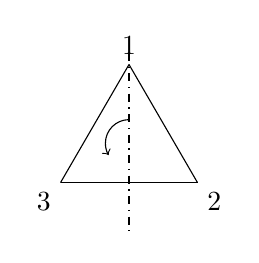
\begin{tikzpicture}
    \coordinate (y) at (0.87, -0.5);
    \coordinate (x) at (0.00, 1.00);
    \coordinate (z) at (-0.87, -0.5);
    \coordinate (Y0) at (0.00, 1.15);
    \coordinate (Y1) at (0.00, -1.15);
    \draw[thin] (x) -- (y);
    \draw[thin] (y) -- (z);
    \draw[thin] (z) -- (x);
    \draw[thin,->] (0,0.3) arc (90:210:0.3);
    \draw[dashdotted] (Y0) -- (Y1);
    \draw (x) node[anchor=south]{$1$};
    \draw (y) node[anchor=north west]{$2$};
    \draw (z) node[anchor=north east]{$3$};
\end{tikzpicture}

                \end{centering}
            \end{figure}
        \end{column}
        \begin{column}{0.33\textwidth}
            \begin{figure}[H]
                \begin{centering}
                    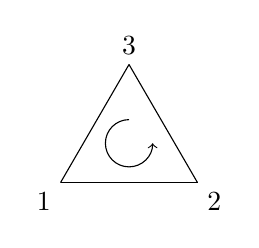
\begin{tikzpicture}
    \coordinate (y) at (0.87, -0.5);
    \coordinate (z) at (0.00, 1.00);
    \coordinate (x) at (-0.87, -0.5);
    \draw[thin] (x) -- (y);
    \draw[thin] (y) -- (z);
    \draw[thin] (z) -- (x);
    \draw[thin,->] (0,0.3) arc (90:360:0.3);
    \draw (x) node[anchor=north east]{$1$};
    \draw (z) node[anchor=south]{$3$};
    \draw (y) node[anchor=north west]{$2$};
\end{tikzpicture}

                \end{centering}
            \end{figure}
            \begin{figure}[H]
                \begin{centering}
                    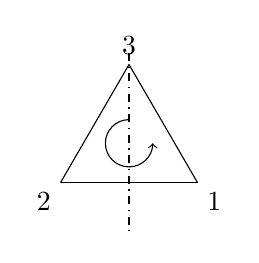
\begin{tikzpicture}
    \coordinate (y) at (0.87, -0.5);
    \coordinate (z) at (0.00, 1.00);
    \coordinate (x) at (-0.87, -0.5);
    \coordinate (Y0) at (0.00, 1.15);
    \coordinate (Y1) at (0.00, -1.15);
    \draw[thin] (x) -- (y);
    \draw[thin] (y) -- (z);
    \draw[thin] (z) -- (x);
    \draw[thin,->] (0,0.3) arc (90:360:0.3);
    \draw[dashdotted] (Y0) -- (Y1);
    \draw (x) node[anchor=north east]{$2$};
    \draw (z) node[anchor=south]{$3$};
    \draw (y) node[anchor=north west]{$1$};
\end{tikzpicture}

                \end{centering}
            \end{figure}
        \end{column}
    \end{columns}
\end{frame}

\begin{frame}
    \frametitle{Перестановки}
    \begin{columns}
        \begin{column}{0.33\textwidth}
            \begin{equation*}
                \left(\begin{array}{ccc}
                    1 & 2 & 3 \\
                    1 & 2 & 3
                \end{array}\right)
            \end{equation*}
            \par\vspace{0.3cm}
            \begin{equation*}
                \left(\begin{array}{ccc}
                    1 & 2 & 3 \\
                    3 & 2 & 1
                \end{array}\right)
            \end{equation*}
        \end{column}
        \begin{column}{0.33\textwidth}
            \begin{equation*}
                \left(\begin{array}{ccc}
                    1 & 2 & 3 \\
                    3 & 1 & 2 
                \end{array}\right)
            \end{equation*}
            \par\vspace{0.3cm}
            \begin{equation*}
                \left(\begin{array}{ccc}
                    1 & 2 & 3 \\
                    2 & 1 & 3
                \end{array}\right)
            \end{equation*}
        \end{column}
        \begin{column}{0.33\textwidth}
            \begin{equation*}
                \left(\begin{array}{ccc}
                    1 & 2 & 3 \\
                    2 & 3 & 1 
                \end{array}\right)
            \end{equation*}
            \par\vspace{0.3cm}
            \begin{equation*}
                \left(\begin{array}{ccc}
                    1 & 2 & 3 \\
                    1 & 3 & 2 
                \end{array}\right)
            \end{equation*}
        \end{column}
    \end{columns}
\end{frame}

\begin{frame}
    \begin{columns}
        \begin{column}{0.33\textwidth}
            \begin{equation*}
                \left(\begin{array}{ccc}
                    1 & 2 & 3 \\
                    1 & 2 & 3
                \end{array}\right)
            \end{equation*}
            \vspace{-0.5cm}
            \begin{figure}[H]
                \begin{centering}
                    \begin{tikzpicture}
    \coordinate (x) at (0.87, -0.5);
    \coordinate (y) at (0.00, 1.00);
    \coordinate (z) at (-0.87, -0.5);
    \draw[thin] (x) -- (y);
    \draw[thin] (y) -- (z);
    \draw[thin] (z) -- (x);
    \draw (x) node[anchor=north west]{$1$};
    \draw (z) node[anchor=north east]{$3$};
    \draw (y) node[anchor=south]{$2$};
\end{tikzpicture}

                \end{centering}
            \end{figure}
            \vspace{-0.2cm}
            \begin{equation*}
                \left(\begin{array}{ccc}
                    1 & 2 & 3 \\
                    3 & 2 & 1
                \end{array}\right)
            \end{equation*}
            \vspace{-0.5cm}
            \begin{figure}[H]
                \begin{centering}
                    \begin{tikzpicture}
    \coordinate (x) at (0.87, -0.5);
    \coordinate (y) at (0.00, 1.00);
    \coordinate (z) at (-0.87, -0.5);
    \coordinate (Y0) at (0.00, 1.15);
    \coordinate (Y1) at (0.00, -1.15);
    \draw[thin] (x) -- (y);
    \draw[thin] (y) -- (z);
    \draw[thin] (z) -- (x);
    \draw[dashdotted] (Y0) -- (Y1);
    \draw (x) node[anchor=north west]{$3$};
    \draw (z) node[anchor=north east]{$1$};
    \draw (y) node[anchor=south]{$2$};
\end{tikzpicture}

                \end{centering}
            \end{figure}
        \end{column}
        \begin{column}{0.33\textwidth}
            \begin{equation*}
                \left(\begin{array}{ccc}
                    1 & 2 & 3 \\
                    3 & 1 & 2 
                \end{array}\right)
            \end{equation*}
            \vspace{-0.5cm}
            \begin{figure}[H]
                \begin{centering}
                    \begin{tikzpicture}
    \coordinate (y) at (0.87, -0.5);
    \coordinate (x) at (0.00, 1.00);
    \coordinate (z) at (-0.87, -0.5);
    \draw[thin] (x) -- (y);
    \draw[thin] (y) -- (z);
    \draw[thin] (z) -- (x);
    \draw[thin,->] (0,0.3) arc (90:210:0.3);
    \draw (x) node[anchor=south]{$1$};
    \draw (y) node[anchor=north west]{$3$};
    \draw (z) node[anchor=north east]{$2$};
\end{tikzpicture}

                \end{centering}
            \end{figure}
            \vspace{-0.2cm}
            \begin{equation*}
                \left(\begin{array}{ccc}
                    1 & 2 & 3 \\
                    2 & 1 & 3
                \end{array}\right)
            \end{equation*}
            \vspace{-0.5cm}
            \begin{figure}[H]
                \begin{centering}
                    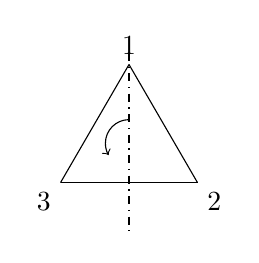
\begin{tikzpicture}
    \coordinate (y) at (0.87, -0.5);
    \coordinate (x) at (0.00, 1.00);
    \coordinate (z) at (-0.87, -0.5);
    \coordinate (Y0) at (0.00, 1.15);
    \coordinate (Y1) at (0.00, -1.15);
    \draw[thin] (x) -- (y);
    \draw[thin] (y) -- (z);
    \draw[thin] (z) -- (x);
    \draw[thin,->] (0,0.3) arc (90:210:0.3);
    \draw[dashdotted] (Y0) -- (Y1);
    \draw (x) node[anchor=south]{$1$};
    \draw (y) node[anchor=north west]{$2$};
    \draw (z) node[anchor=north east]{$3$};
\end{tikzpicture}

                \end{centering}
            \end{figure}
        \end{column}
        \begin{column}{0.33\textwidth}
            \begin{equation*}
                \left(\begin{array}{ccc}
                    1 & 2 & 3 \\
                    2 & 3 & 1 
                \end{array}\right)
            \end{equation*}
            \vspace{-0.5cm}
            \begin{figure}[H]
                \begin{centering}
                    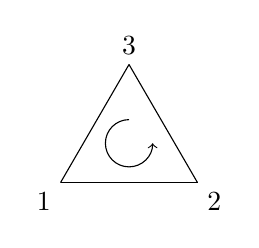
\begin{tikzpicture}
    \coordinate (y) at (0.87, -0.5);
    \coordinate (z) at (0.00, 1.00);
    \coordinate (x) at (-0.87, -0.5);
    \draw[thin] (x) -- (y);
    \draw[thin] (y) -- (z);
    \draw[thin] (z) -- (x);
    \draw[thin,->] (0,0.3) arc (90:360:0.3);
    \draw (x) node[anchor=north east]{$1$};
    \draw (z) node[anchor=south]{$3$};
    \draw (y) node[anchor=north west]{$2$};
\end{tikzpicture}

                \end{centering}
            \end{figure}
            \vspace{-0.2cm}
            \begin{equation*}
                \left(\begin{array}{ccc}
                    1 & 2 & 3 \\
                    1 & 3 & 2 
                \end{array}\right)
            \end{equation*}
            \vspace{-0.5cm}
            \begin{figure}[H]
                \begin{centering}
                    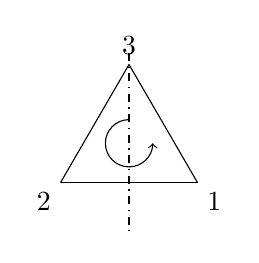
\begin{tikzpicture}
    \coordinate (y) at (0.87, -0.5);
    \coordinate (z) at (0.00, 1.00);
    \coordinate (x) at (-0.87, -0.5);
    \coordinate (Y0) at (0.00, 1.15);
    \coordinate (Y1) at (0.00, -1.15);
    \draw[thin] (x) -- (y);
    \draw[thin] (y) -- (z);
    \draw[thin] (z) -- (x);
    \draw[thin,->] (0,0.3) arc (90:360:0.3);
    \draw[dashdotted] (Y0) -- (Y1);
    \draw (x) node[anchor=north east]{$2$};
    \draw (z) node[anchor=south]{$3$};
    \draw (y) node[anchor=north west]{$1$};
\end{tikzpicture}

                \end{centering}
            \end{figure}
        \end{column}
    \end{columns}
\end{frame}

\subsection{Непрерывные симметрии}
\begin{frame}
    \frametitle{Тела вращения}
    \begin{columns}
        \begin{column}{0.5\textwidth}
            \begin{figure}
                \begin{centering}
                    \includegraphics[width=0.99\textwidth]{sphere}
                \end{centering}
            \end{figure}
        \end{column}
        \begin{column}{0.5\textwidth}
            \begin{figure}
                \begin{centering}
                    \includegraphics[width=0.5\textwidth]{cylinder}
                \end{centering}
            \end{figure}
        \end{column}
    \end{columns}
\end{frame}

\subsection{Симметрии в физике}
\begin{frame}
    \frametitle{Стандартная модель ФЭЧ}
    \begin{figure}
        \begin{centering}
            \includegraphics[width=0.7\textwidth]{sm}
        \end{centering}
    \end{figure}
\end{frame}
